\begin{figure}[!htb]
\begin{center}
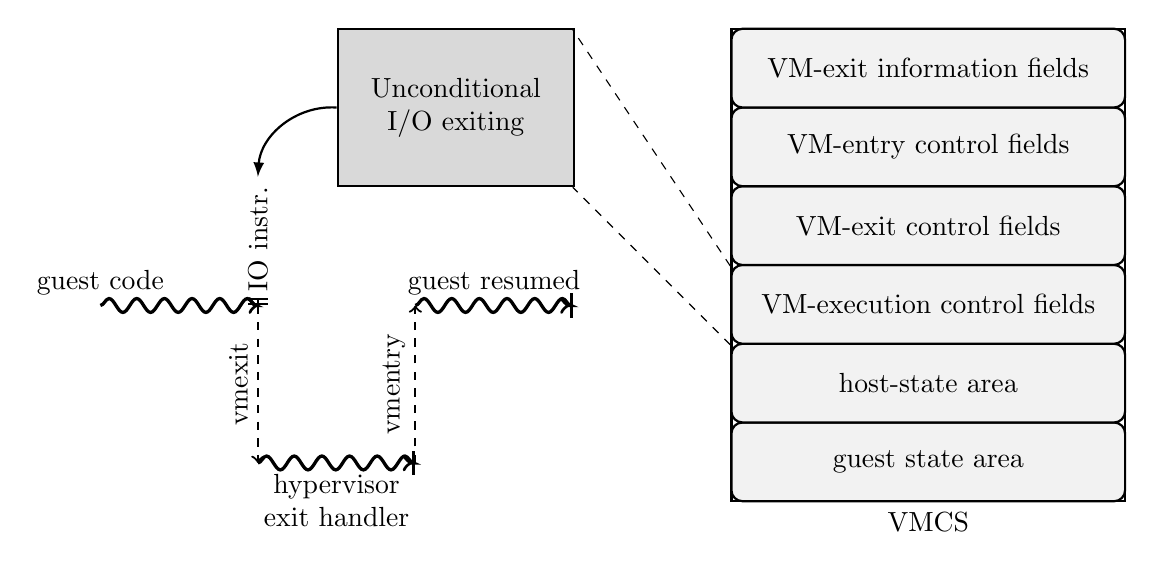
\begin{tikzpicture}

%\draw[step=0.5cm, gray, very thin] (0,0) grid (9,9)


\draw[very thick, decorate, decoration=snake, ->] (0, 2.5) -- (2, 2.5) node at (0,2.5) [above] {guest code};
\draw[thick, |-|] (2, 2.5) -- (2, 2.6) node at (2, 2.6)[right, midway, rotate=90] (ioinst) {IO instr.};

\draw[very thick, decorate, decoration=snake, ->|] (2, 0.5) -- (4, 0.5) node [below, midway, align=center] {hypervisor\\ exit handler};
\draw[very thick, decorate, decoration=snake, ->|] (4, 2.5) -- (6, 2.5) node [above, align=center, midway] {guest resumed};

\draw[thick, dashed, ->] (2, 2.5) -- (2, 0.5) node [above, align=center,midway, rotate=90] {vmexit};
\draw[thick, dashed, ->] (4, 0.5) -- (4, 2.5) node [above, align=center,midway, rotate=90] {vmentry};


\node at (3,4) [rectangle, draw=black, thick, fill=black!15, minimum height = 2cm, minimum width = 3cm, anchor=south west, align=center] (exitcontrol) 
                        {Unconditional\\ I/O exiting} ;


\node at (8,0) [rectangle, draw=black, thick, fill=white, minimum height = 6cm, minimum width = 5cm, anchor=south west] (vmcs) {} ;
\node [below, align=center] at (vmcs.south) {VMCS};
%\node[below right, inner sep=5pt, text width=2cm] at (rtguest.north west) {PREEMPT\_RT\\ Linux\\ (rt-guest)};


\node at (8,0) [rectangle, draw=black, thick, rounded corners, fill=black!5, minimum height = 1cm, minimum width = 5cm, anchor=south west] (gstate) {guest state area};
\node at (8,1) [rectangle, draw=black, thick, rounded corners, fill=black!5, minimum height = 1cm, minimum width = 5cm, anchor=south west] (gstate) {host-state area};
\node at (8,2) [rectangle, draw=black, thick, rounded corners, fill=black!5, minimum height = 1cm, minimum width = 5cm, anchor=south west] (gstate) {VM-execution control fields};
\node at (8,3) [rectangle, draw=black, thick, rounded corners, fill=black!5, minimum height = 1cm, minimum width = 5cm, anchor=south west] (gstate) {VM-exit control fields};
\node at (8,4) [rectangle, draw=black, thick, rounded corners, fill=black!5, minimum height = 1cm, minimum width = 5cm, anchor=south west] (gstate) {VM-entry control fields};
\node at (8,5) [rectangle, draw=black, thick, rounded corners, fill=black!5, minimum height = 1cm, minimum width = 5cm, anchor=south west] (gstate) {VM-exit information fields};

\draw [dashed] (8,2) -- (6,4); 
\draw [dashed] (8,3) -- (6,6); 

\begin{scope}[>=latex]
	\draw [thick, ->] (exitcontrol.west) to [bend right=45] (ioinst.east);
\end{scope}

\end{tikzpicture}
\end{center}
\ifreport
\caption{VMCS data structure with an example of using VMCS fields to control guest execution behavior}
\fi
\label{fig-vmcs-ds}
\end{figure}
